% !TeX spellcheck = sv_SE
\documentclass[a4paper,11pt,twoside]{report}
\usepackage[swedish]{babel}
\usepackage{t1enc}
\usepackage[dvips]{graphicx}
\usepackage{listings}
\usepackage{color}

\usepackage{amsthm}
\usepackage{bbm}
\usepackage{graphicx}

\DeclareGraphicsExtensions{.png,.pdf,.jpg}

\textheight=24.0cm
\textwidth=15.1cm

\topmargin=-1.5cm
%\headheight=0cm
\headsep=0.7cm
\oddsidemargin=0.4cm
\evensidemargin=0.4cm
%\columnsep=0.8cm
\footskip=1.5cm
\setcounter{secnumdepth}{0}
\pagestyle{empty}
%\markboth{}{Namn: \hfill Personnr: \hfill}
%\markboth{DD1339 inda13}{DD1339 inda13}

\newcommand{\ttt}[1]{\texttt{#1}}

\definecolor{codegreen}{rgb}{0,0.6,0}
\definecolor{codegray}{rgb}{0.5,0.5,0.5}
\definecolor{codepurple}{rgb}{0.58,0,0.82}
\definecolor{backcolour}{rgb}{0.95,0.95,0.92}

\lstdefinestyle{mystyle}{
	language=C,
	commentstyle=\color{codegreen},
	keywordstyle=\color{magenta},
	numberstyle=\tiny\color{codegray},
	stringstyle=\color{codepurple},
	basicstyle=\footnotesize,
	breakatwhitespace=false,         
	breaklines=true,                 
	captionpos=b,                    
	keepspaces=true,                 
	numbers=left,                    
	numbersep=5pt,
	rulecolor=\color{black},                  
	showspaces=false,                
	showstringspaces=false,
	showtabs=false,
	stepnumber=2,                  
	tabsize=2
}

\lstset{style=mystyle}

\begin{document}

\section{Programbeskrivning}
Programmet kommer att vara ett enkelt tv�personsspel.
Spelet kommer i grunden att g� ut p� att man styr varsitt piratskepp och f�rs�ker skjuta ner varandra.

\subsection{Syfte}
Spelets syfte �r att vara ett kul socialt tidsf�rdriv.

Vi har valt att g�ra detta spel, d� vi minns fr�n v�r ungdoms dagar hur roligt det var att spela flashspelet ''achtung die kurve'' och vill �terskapa gl�djen av att sitta ett g�ng kompisar runt en dator och skrika p� varandra.

\section{Anv�ndare}
Vi riktar oss mot andra studenter och spelintresserade som vill ha ett kul tidsf�rdriv.

Vi f�rv�ntar oss att anv�ndarna har spelat enkla flash-spel f�rut och klarar av att navigera i en simpel meny. Inte s� mycket allts�.

\section{Anv�ndarscenarion}
Tv� anv�ndare sitter efter lunch och har inget att g�ra, s� de best�mmer sig f�r att spela v�rt spel. De s�tter sig vid en dator och startar en spelomg�ng. Vid datorns tangentbord har de varsin upps�ttning knappar f�r att navigera och skjuta. Efter att ha skjutit och rammat varandra ett tag s� f�r en av anv�ndarna slut p� hitpoints och hans skepp sjunker och han f�rlorar. Efter matchen fr�gar programmet om de vill k�ra en till omg�ng men anv�ndarna best�mmer sig f�r att g�ra n�got annat s� de st�nger ner programmet.
\begin{figure}[h!]
	\centering
	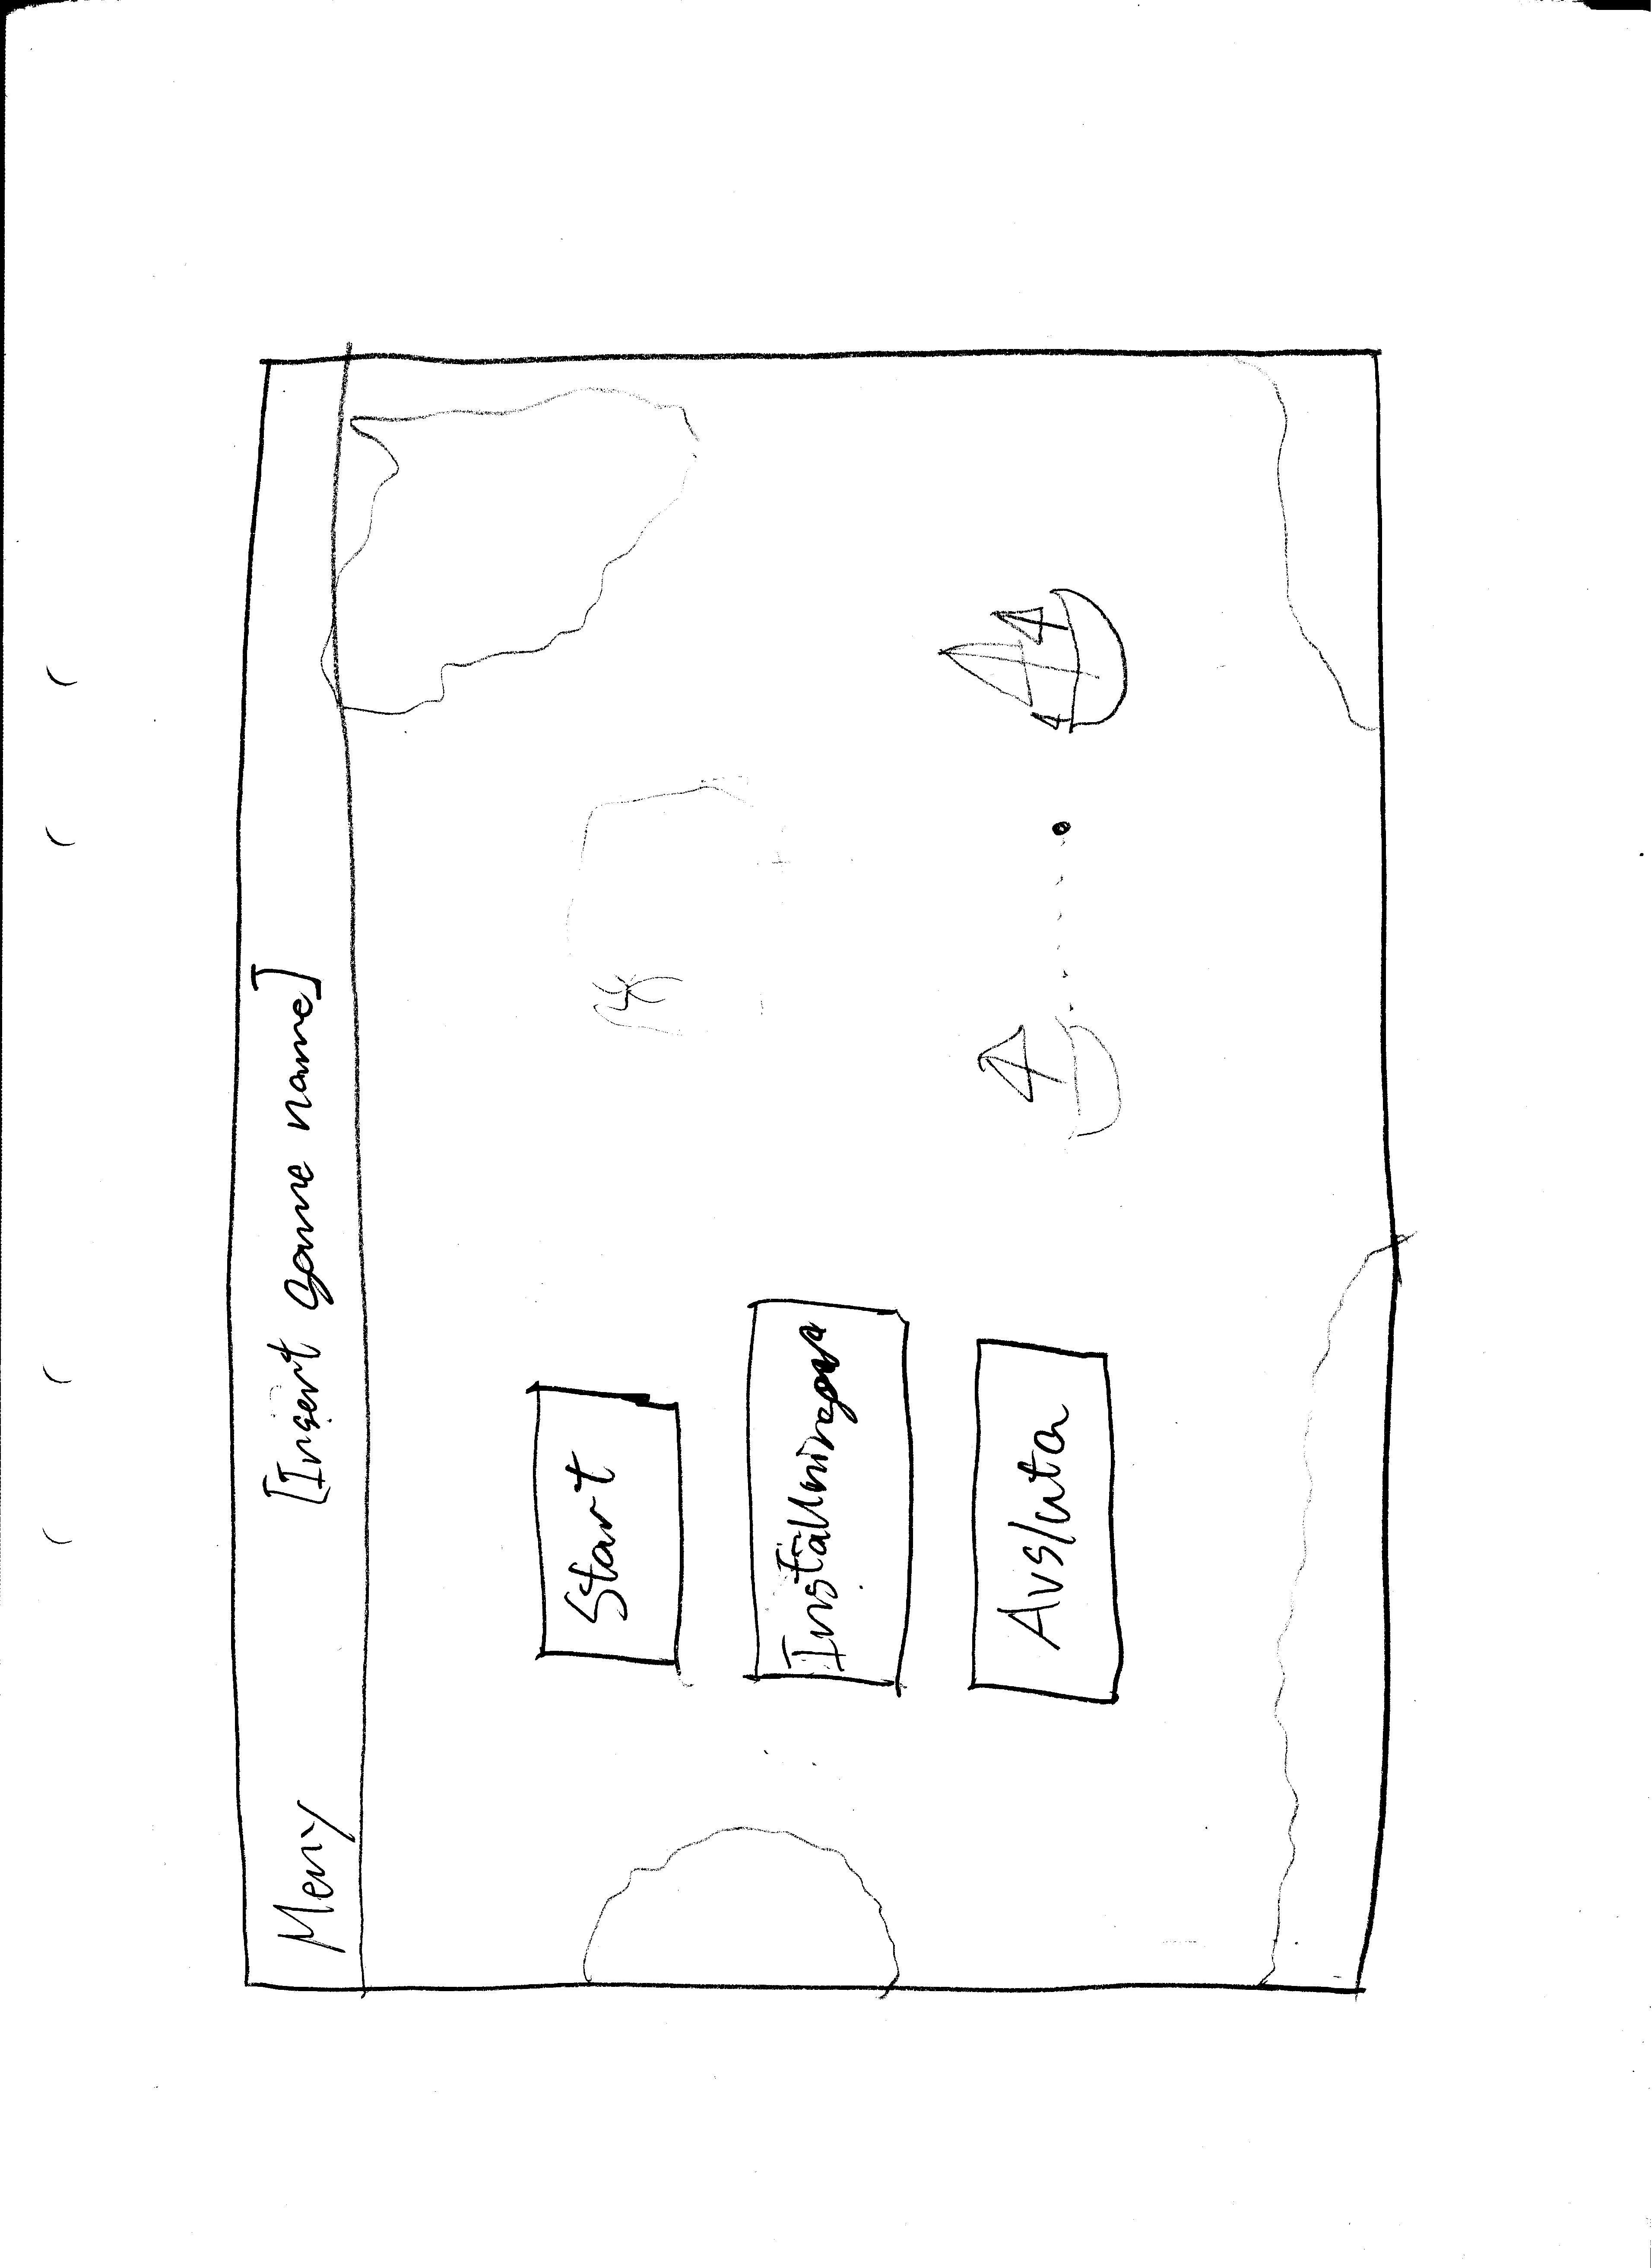
\includegraphics[width=0.3\textwidth , angle=270]{Bilder/Meny}
	%\caption{Spelets huvudmeny}
	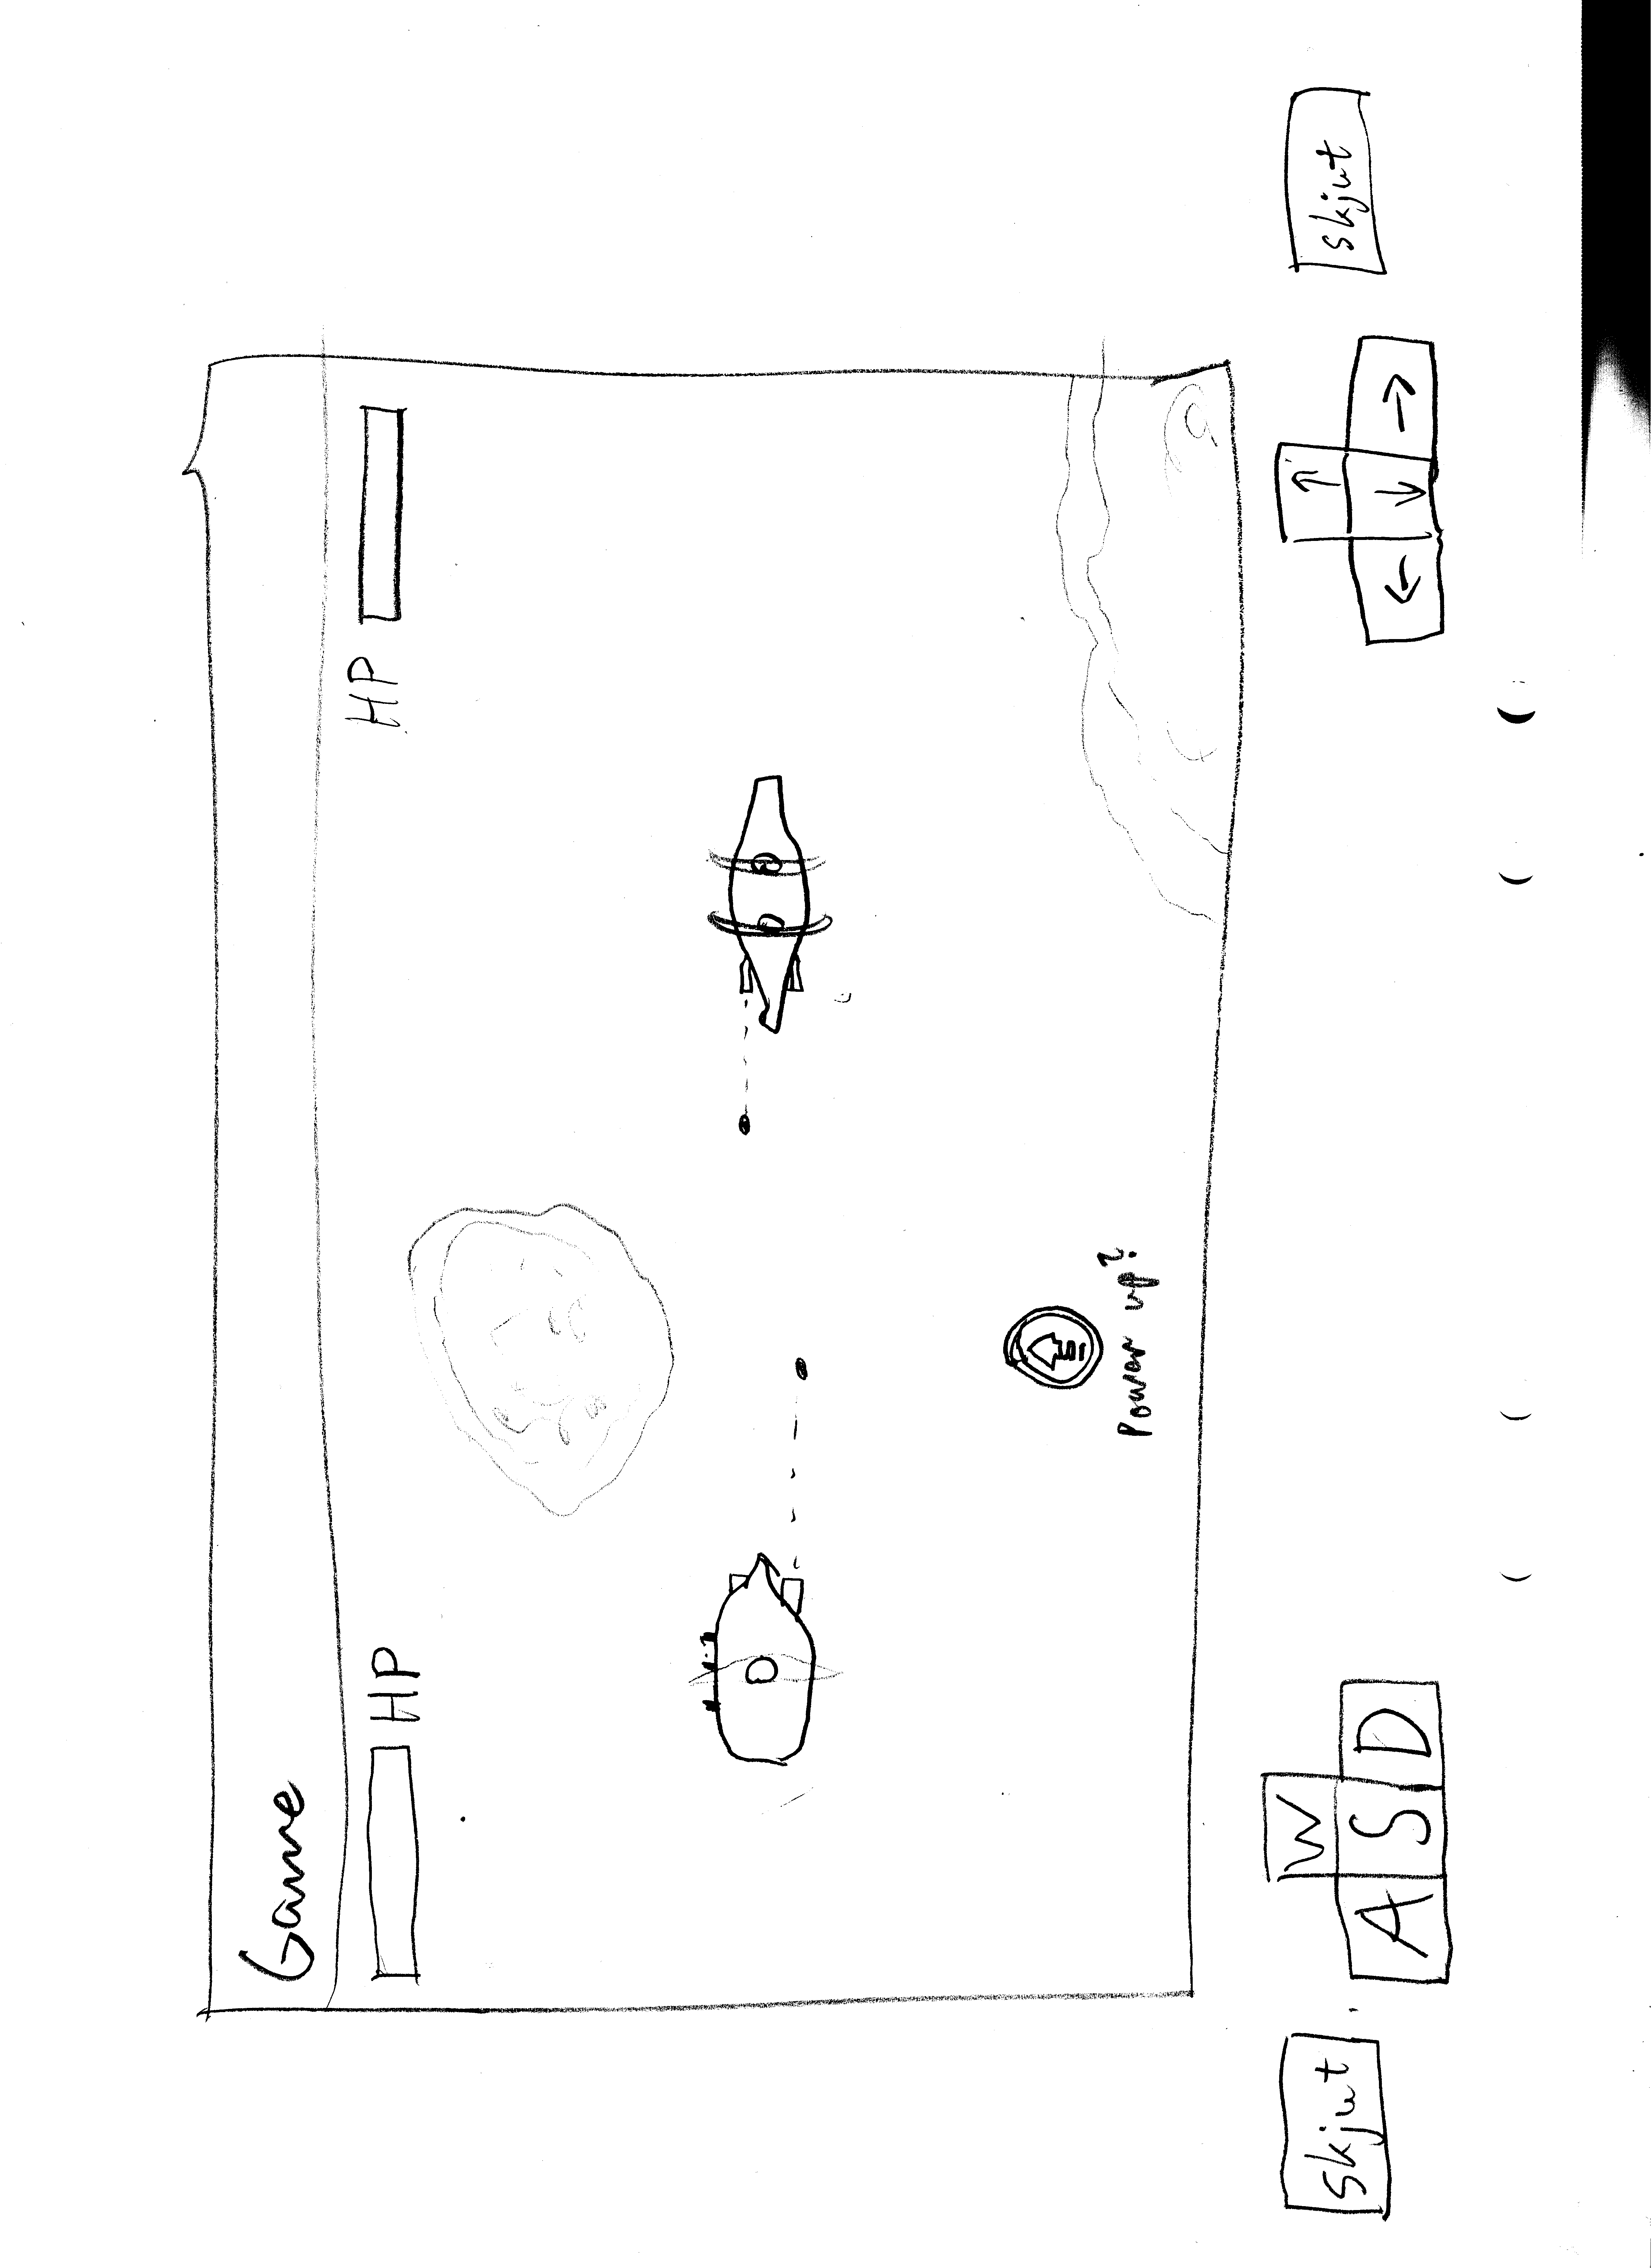
\includegraphics[width=0.3\textwidth , angle=270]{Bilder/Game}
	\caption{Huvudmeny och spelplan}
\end{figure}

\section{Testplan}


\section{Programdesign}


\section{Tekniska specifikationer}


\section{Tidsplan}


\end{document}
